\documentclass[a4paper,12pt]{article}

\usepackage{fancyhdr}
\usepackage{lastpage}
\usepackage{amsmath}
\usepackage{tikz}
\usepackage{amsfonts}
\usepackage{graphicx}
\usepackage{float}

\newcommand{\V}[1]{\ensuremath{\vec{#1}}}
\newcommand{\F}[2]{\ensuremath{\frac{#1}{#2}}}
\newcommand{\Q}[1]{\newpage \section*{#1}}
\newcommand{\acc}[1]{\overset{..}{#1}}
\newcommand{\vel}[1]{\overset{.}{#1}}
\newcommand{\prt}[2]{\frac{\partial#1}{\partial#2}}
\newcommand{\LP}{\left(}
\newcommand{\RP}{\right)}


\pagestyle{fancy}
\lhead{Samuel Loomis}
\setlength{\headheight}{15pt}
\chead{PH 411 Lab 2}
\rhead{15 November 2013}
\lfoot{}
\cfoot{\thepage\ of \pageref{LastPage}}
\rfoot{}

\begin{document}

\section*{Homework}
\subsection*{Simpson 2.4}
Calculate the capacitance in microfarads between two 1-cm$^2$ conducting plates 1 mm apart in a vacuum.  Repeat if the space between the plates is filled with a plastic dielectric with a dielectric constant of 8.
\\
\\
The formula for calculating capacitance is:
\[C=\epsilon_0\F{A}{d}\]
The area ($A$) is $1-cm^2=(0.01m)^2=0.0001m^2$.\\
The distance apart ($d$) is $ 1-mm=0.001-m$.\\
$\epsilon_0=8.85\cdot10^{-12}\F{F}{m}$.
\begin{align*}
C&=8.85\cdot10^{-12}\F{F}{m}\F{0.0001m^2}{0.001-m}\\
&=8.85\cdot10^{-13}F\\
&=8.85\cdot10^{-7}\mu F
\end{align*}
\subsection*{Simpson 2.8}
Calculate the energy in joules stored in a 2000-$\mu$F capacitor charged to 5V. Physically, how is the energy stored?
\\
\\
The formula for energy stored in a capacitor is:
\[W=\F{1}{2}CV^2\]
$C=2000-\mu F=2\cdot10^{-3}F$, $V=5V$ so the energy in Joules is:
\begin{align*}
W&=\F{1}{2}\cdot2\cdot10^{-3}F\cdot(5V)^2\\
&=2.5\cdot10^{-2}J
\end{align*}
The energy is stored in the electric field between the two oppositly charged plates.

\subsection*{Simpson 2.10}
Calculate the impedance $Z$ in the form $a+jb$ and $|Z|e^{j\theta}$ for\\
\begin{figure}[H]
\centering
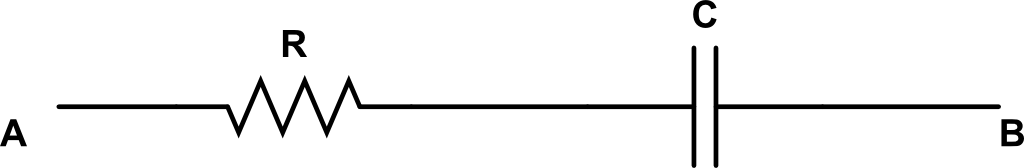
\includegraphics[width=2.5in]{sam_lab2/simpson_rc_series.png}
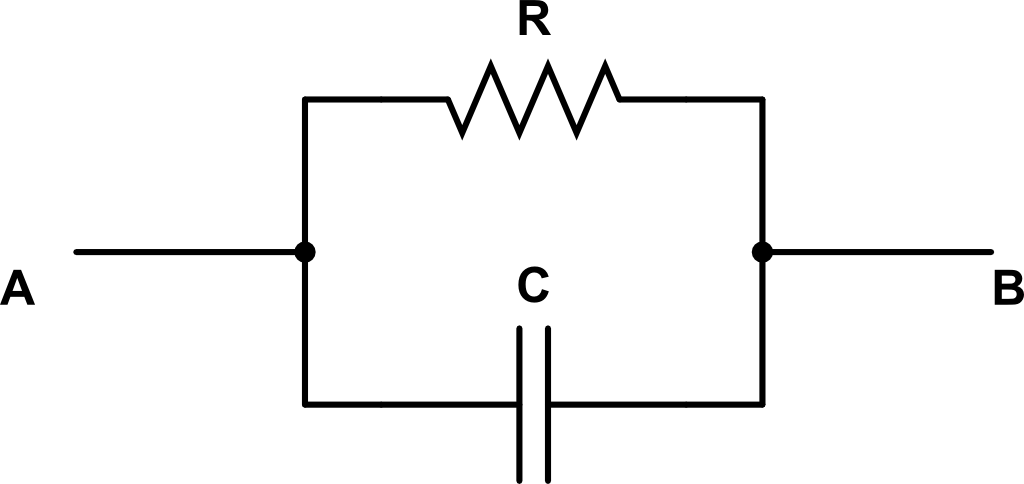
\includegraphics[width=2in]{sam_lab2/simpson_rc_parallel.png}
\caption{RC in series(left) and parallel(right).}
\end{figure}
\noindent
The impedance of a resistor is R, and the impedance of a capacitor is $\F{-j}{\omega C}$.  For the series circuit shown, the impedances are directly added:
\begin{align*}
Z&=R+\F{-j}{\omega C}\\
a+jb&=R+j\LP\F{-1}{\omega C}\RP\\
\end{align*}
For the $|Z|e^{j\theta}$ form, the magnitude $|Z|= \sqrt{a^2+b^2}$ and there is a $\phi$ term that equals $arctan{\F{b}{a}}$:
\[Z=\sqrt{R^2+\F{1}{(\omega C)^2}}e^{j(\theta-arctan\LP\F{1}{\omega RC}\RP)}\]
For the parallel circuit shown, the impedances add similar to parallel resistors:
\begin{align*}
Z_\parallel&=\F{Z_1Z_2}{Z_1+Z_2}\\
&=\F{\F{-jR}{\omega C}}{R-\F{j}{\omega C}}
\end{align*}
Multiplying top and bottom by the complex conjugate of the bottom gives:
\begin{align*}
Z_\parallel&=\F{\F{R}{\omega^2C^2}-\F{jR^2}{\omega C}}{R^2+\F{1}{\omega^2C^2}}\\
&=\F{R-jR^2\omega C}{R^2\omega^2C^2+1}
\end{align*}
The exponential form is:
\[Z_\parallel=\F{\sqrt{R^2+R^4\omega^2C^2}}{R^2\omega^2C^2+1}e^{j(\theta-arctan(R\omega C))}\]


\subsection*{Simpson 2.14}
Design a low-pass RC filter that will attenuate a 60-Hz sinusoidal voltage by 12 dB relative to the dc gain.  Use a 100-$\Omega$ resistance. Explain in words why the low-pass RC filter attenuates the high frequencies.\\
\\
The circuit will look like this:
\begin{figure}[h]
\centering
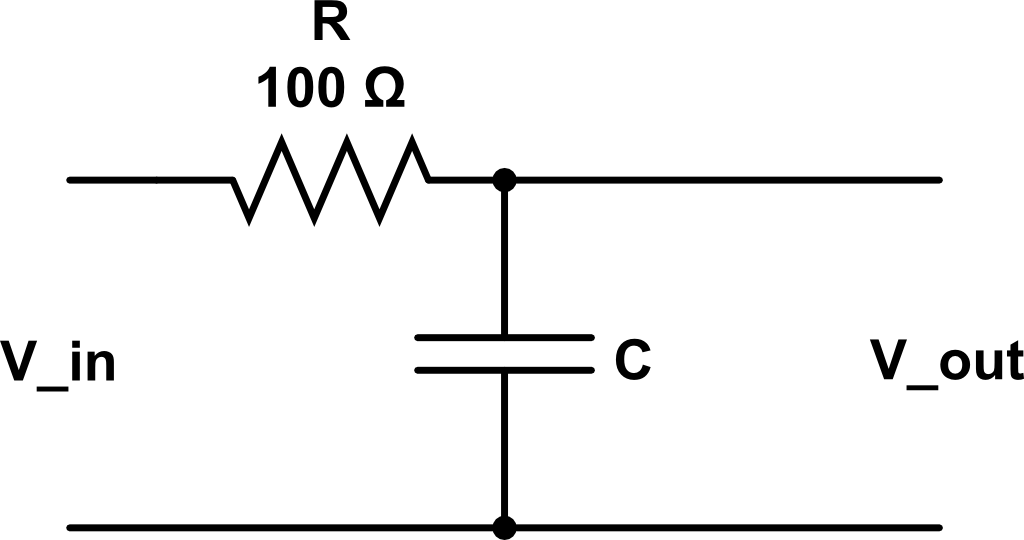
\includegraphics[width=2in]{sam_lab2/simpson_low_pass.png}
\caption{Low-pass circuit.}
\end{figure}
This circuit will act like a voltage divider with a complex impedance.  The ratio of $V_{out}$ and $V_{in}$ will be equal to the ratio of the complex impedance of the capacitor to the total complex impedance of the circuit:
\[\F{V_{out}}{V_{in}}=\F{\F{-j}{\omega C}}{R-\F{j}{\omega C}}=\F{1}{1+j\omega RC}\]
To find the capacitor value needed to create this specific low pass circuit, the magnitude of this ratio needs to be found:
\[\left|\F{V_{out}}{V_{in}}\right|=\left[\LP\F{1}{1-j\omega RC}\RP\LP\F{1}{1+j\omega RC}\RP\right]^{\F{1}{2}}=\F{1}{\sqrt{1+\omega^2R^2C^2}}\]
The voltage gain in decibals is:
\[\LP\F{V_{out}}{V_{in}}\RP_{in~dB}=20log\LP\F{V_{out}}{V_{in}}\RP\]
The capacitor needed to achieve a 12 dB attenuation will be the capacitor that solves this equation:
\[20log\left[\F{1}{\sqrt{1+\omega^2R^2C^2}}\right]=-12\]
Solving for C:
\begin{align*}
20log\left[\F{1}{\sqrt{1+\omega^2R^2C^2}}\right]&=-12\\
\F{1}{\sqrt{1+\omega^2R^2C^2}}&=10^{\F{-3}{5}}\\
10^{\F{6}{5}}&=1+\omega^2R^2C^2\\
\F{10^{\F{6}{5}}-1}{\omega^2R^2}&=C^2\\
\sqrt{\F{10^{\F{6}{5}}-1}{\omega^2R^2}}&=C\\
C&=\sqrt{\F{10^{\F{6}{5}}-1}{60^2\cdot100^2}}\approx 642\mu F
\end{align*}
This tells me that the breakpoint frequency of a low pass circuit made with a 100 $\Omega$ resistor and a 642 $\mu F$ capacitor should be about 20 Hz.
\subsection*{Simpson 2.22}
Sketch the approximate gain-versus-frequency curve for the following circuit.  You may treat the circuit as being composed of two independent RC filters.

\begin{figure}[h]
\centering
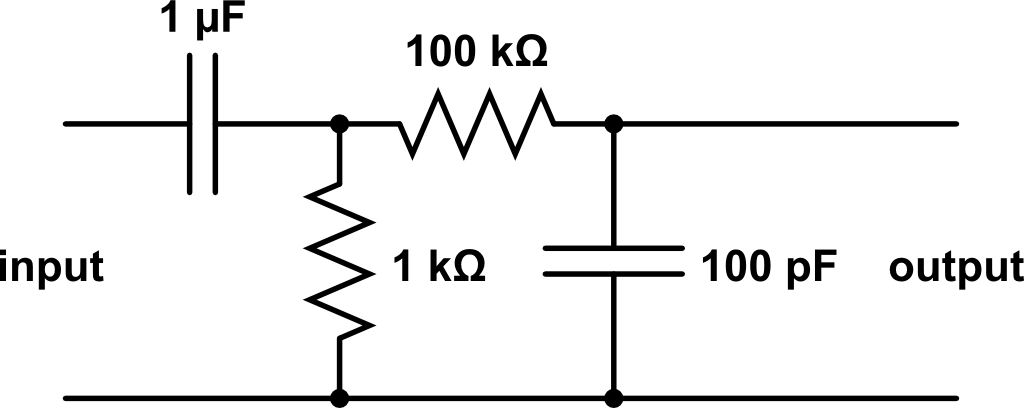
\includegraphics[width=2.5in]{sam_lab2/simpson_high_low.png}
\caption{High-pass circuit combined with a low-pass circuit.}
\end{figure}
\noindent
If just the high pass circuit existed, the gain-versus-frequency curve would start out low and increase at a rate of 6 dB per octave untill the high-pass breakpoint frequency and taper off twords 0 dB.  If just the low pass circuit existed, the gain-versus-frequency curve would start out at 0 dB and slowly taper down till it reaches -3 dB at the low-pass breakpoint frequency and then fall at a rate of 6 dB per octave afterwards.  Combining the two types in one circuit will attenuate both the low and the high frequencies and let most of the voltage through inbetween the two breakpoint frequencies.
\\
\\
Finding the breakpoint frequencies will show where to plot the interesting charactersitics described.
\\
\\
Both frequencies can be approximated using:
\[\omega=\F{1}{RC}\]
High-pass breakpoint ($\omega_{h}$):
\[\omega_h=\F{1}{1k\Omega\cdot1\mu F}=1000Hz\]
Low-pass breakpoint ($\omega_l$):
\[\omega_l=\F{1}{100k\Omega\cdot100pF}=100000Hz\]
Here is a plot generated by python:
\begin{figure}[h]
\centering
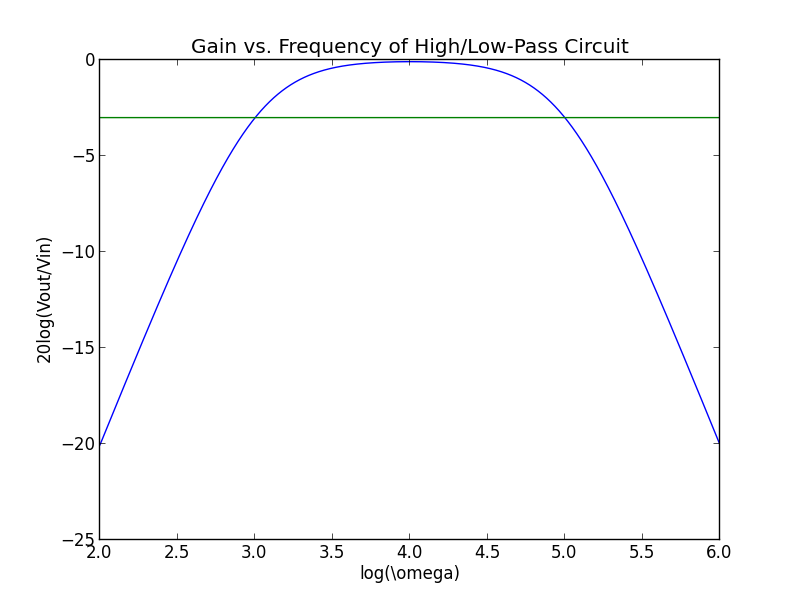
\includegraphics[width=3in]{sam_lab2/log_log.png}
\caption{Python generated plot of the Gain vs. Frequency of the High/Low-pass combination circuit.  The green line shows the -3 dB point and crosses the curve at the breakpoint frequencies, 1 kHz and 100 kHz, as expected.}
\end{figure}  
\newpage
\section*{Lab Experiment 2}
\subsection*{Theoretical}
\begin{figure}[h]
\centering
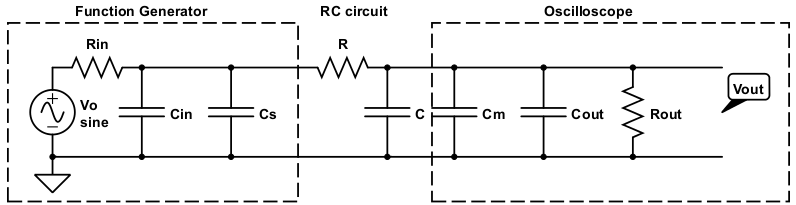
\includegraphics[width=4in]{sam_lab2/effective_rc_circuit.png}
\caption{Circuit diagram for the effective capacitor and resistor layouts of a Function Generator and an Oscilloscope attached to the RC circuit being evaluated.}
\end{figure}
\noindent
$V_{out}$ will be the voltage applied across the resistor($R_{out}$) and the three capacitors, ($C,C_{m},C_{out}$)\\
\\
Finding the impedance $Z_{out}$:
\begin{align*}
Z_{out}&=\F{1}{\F{1}{\F{-j}{\omega C}}+\F{1}{\F{-j}{\omega C_m}}+\F{1}{\F{-j}{\omega C_{out}}}+\F{1}{R_out}}\\
&=\F{1}{\F{1}{R_{out}}-\omega\F{C+C_m+C_{out}}{j}}\\
&=\F{jR_{out}}{j-R_{out}\omega(C+C_m+C_{out})}\\
&=\F{R_{out}-jR_{out}^2\omega(C+C_m+C_{out})}{1+R_{out}^2\omega^2(C+C_m+C_{out})^2}
\end{align*}
$Z_{out}$ is in series with the resistor $R$ and the voltage drop across this combo, and the two capacitors($C_{in}, C_s$) is $V_a$.\\
\\
Finding the impedance $Z_a$:
\begin{align*}
Z_a&=\F{1}{\F{1}{\F{-j}{\omega C_{in}}}+\F{1}{\F{-j}{\omega C_s}}+\F{1}{R+Z_{out}}}\\
&=\F{1}{\F{1}{R+Z_{out}}-\omega\F{C_{in}+C_s}{j}}\\
&=\F{j(R+Z_{out})}{j-\omega(R+Z_{out})(C_{in}+C_s)}
\end{align*}
Before taking the complex conjugate of this step, substituting $Z_{out}$ back into the expression, because it itself is complex and needs to be accounted for.\\
\\
Substituting $Z_{out}$ back in:
\[Z_a=\F{j\LP R+\F{R_{out}-jR_{out}^2\omega(C+C_m+C_{out})}{1+R_{out}^2\omega^2(C+C_m+C_{out})^2}\RP}{j-\omega\LP R+\F{R_{out}-jR_{out}^2\omega(C+C_m+C_{out})}{1+R_{out}^2\omega^2(C+C_m+C_{out})^2}\RP(C_{in}+C_s)}\]
This is looking really messy. Simplifying:
\begin{align*}
C_{in}+C_s&=C_1\\
C+C_m+C_{out}&=C_2\\
R+Z_{out}&=\F{R+R_{out}+RR_{out}^2\omega^2C_2^2-jR_{out}^2\omega C_2}{1+R_{out}^2\omega^2C_2^2}\\
Z_a&=\F{j(R+R_{out}+RR_{out}^2\omega^2C_2^2-jR_{out}^2\omega C_2)}{j(1+R^2\omega^2C_2^2)-\omega C_1(R+R_{out}+RR_{out}^2\omega^2C_2^2-JR_{out}^2\omega C_2)}\\
\end{align*}
At this point, I will come back to this derivation if I have time, However, $V_{out}$ will be equal to:
\[V_{out}=V_{in}\F{Z_aZ_{out}}{(R_{in}+Z_a)(R+Z_{out})}\]
Keep in mind that the expression is complex, and the exponential form will look something like this:
\[V_{out}=V_{in}\sqrt{Real^2+Imaginary^2}e^{i(\theta-arctan\LP\F{Imaginary}{Real}\RP)}\]
\newpage
\subsection*{Experiment}
\begin{figure}[h]
\centering
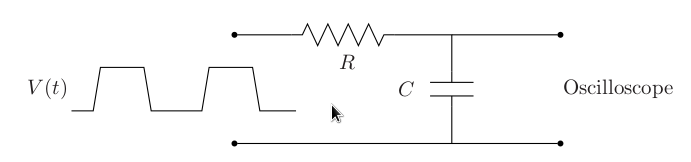
\includegraphics[width=4in]{sam_lab2/lab2_experiment_2.png}
\caption{Square wave applied to a low pass RC circuit.}
\end{figure}
\noindent
A 200$\Omega$ resistor and a 474$\mu F$ capacitor were chosen to make a time constant of $\approx$ 0.0001 seconds.  The time constant $\tau$ is equal to the resistance times the capacitance.  The values obtained for the resistance and capacitance of the function generator, oscilloscope, and cables should have been used, however, they were neglected in the selection of the resistor and capacitor used. This will likely result in a time constant that doesn't match the goal.
\\
\\
A 100Hz square wave was applied to the circuit shown above.  The input and output waves are shown here:
\begin{figure}[h]
\centering
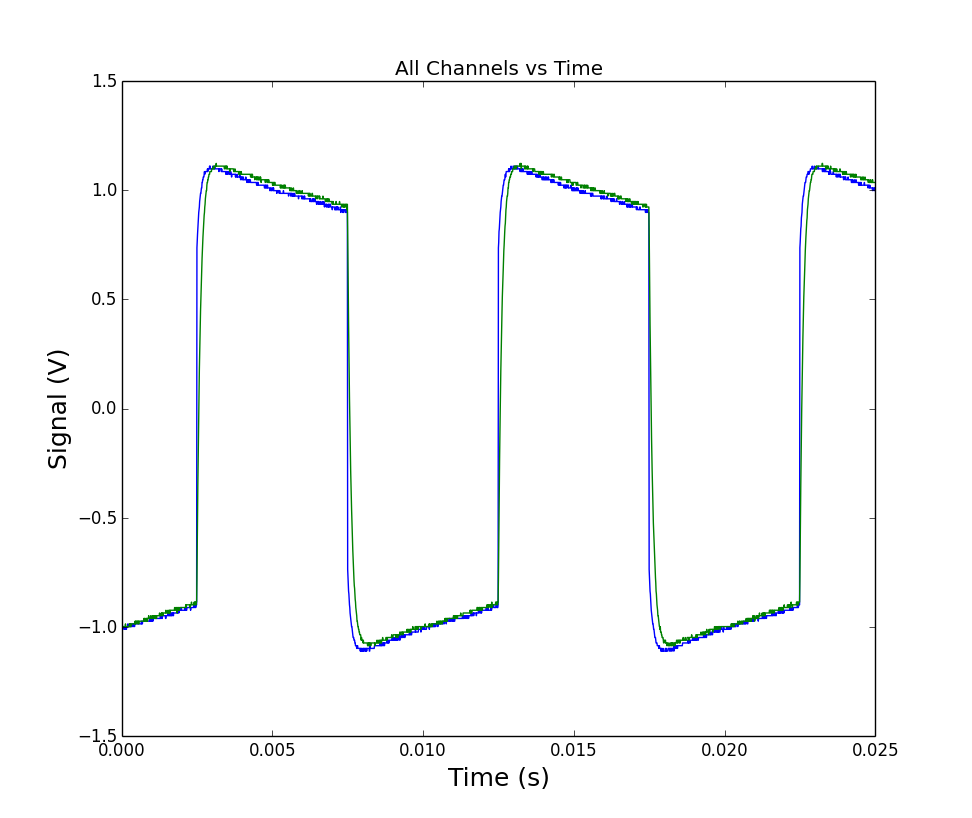
\includegraphics[width=1.5in]{sam_lab2/2e_waveform.png}
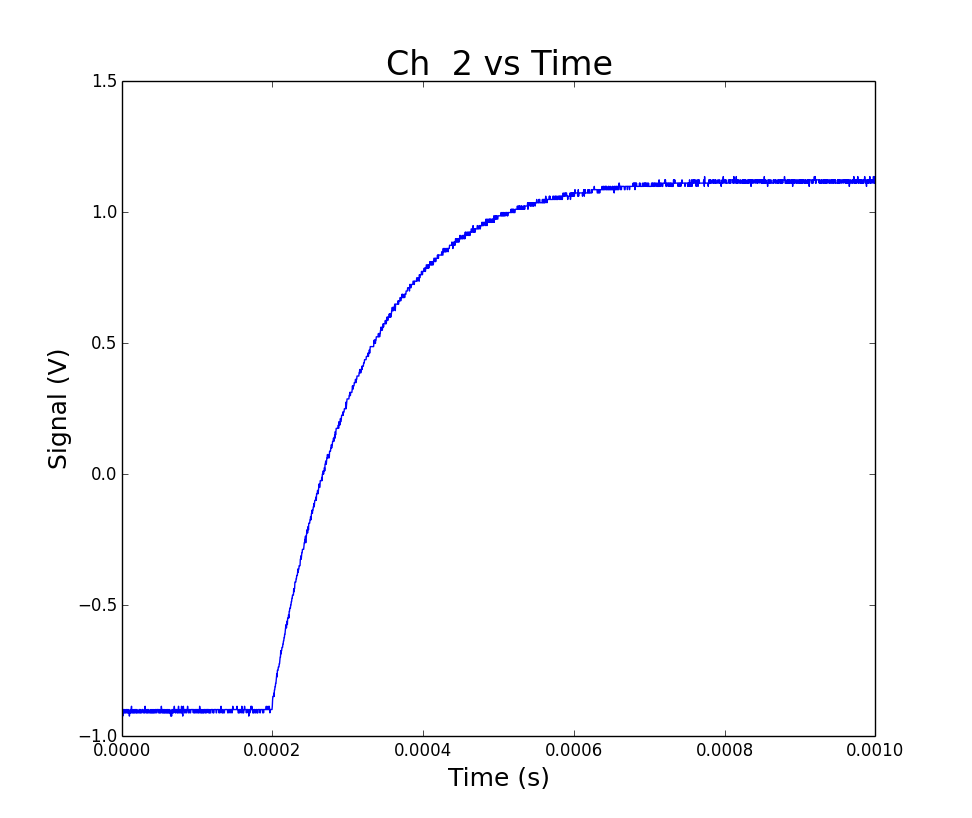
\includegraphics[width=1.5in]{sam_lab2/2e_rise.png}
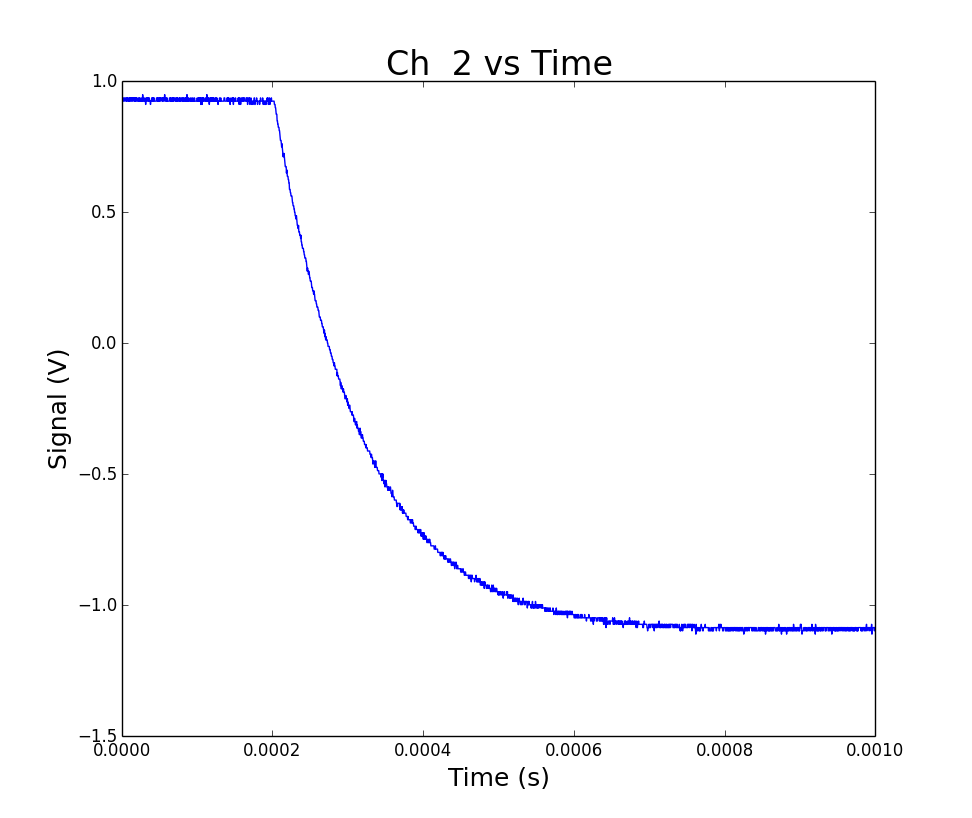
\includegraphics[width=1.5in]{sam_lab2/2e_fall.png}
\caption{100Hz square wave applied to a low pass RC circuit $\tau\approx0.0001$.}
\end{figure}
Cursors on the oscilloscope were used to determing the rise and fall times of the output wave.  The time it takes the capacitor to charge up to $\F{V_{max}}{e}$ is the rise time and should be equal to the time constant. The rise and fall times were both found to be about $50\pm5\mu s$.  This shows that better care should have been taken in choosing the resistor and capacitor.  The time constant measured is about half the time constant expected.
\\
\\
In order to observe the behavior of this circuit, the function generator was then varried from 0 to 100 kHz.\newpage  \noindent Here are some traces:\\
\begin{figure}[h]
\centering
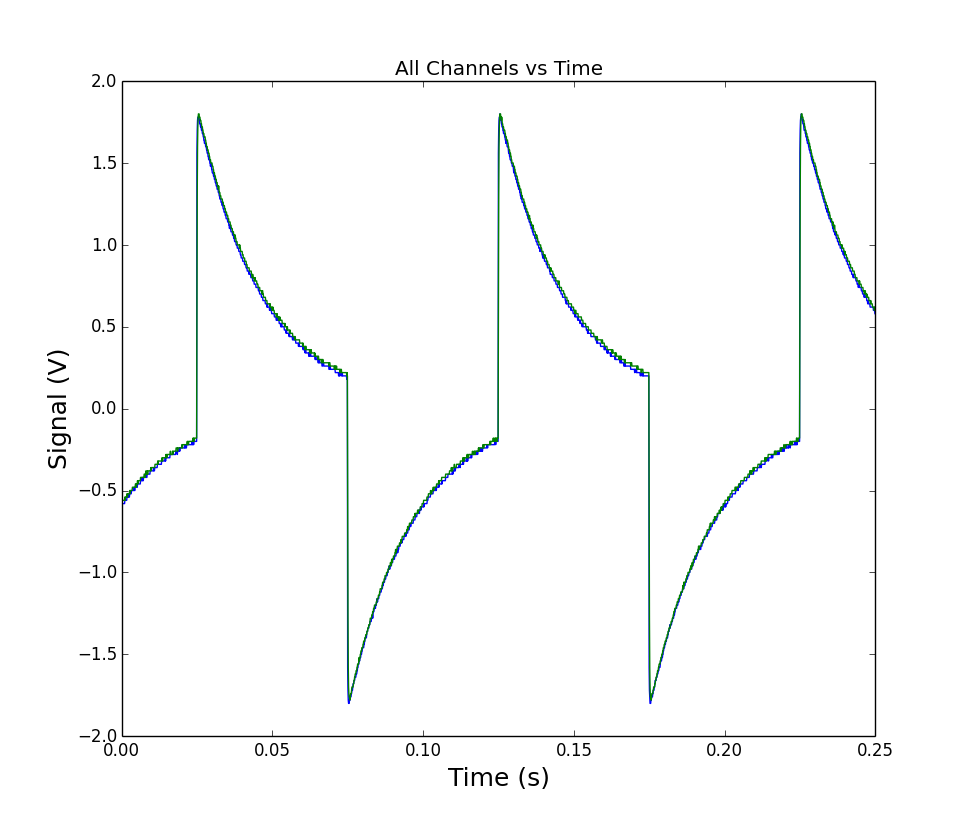
\includegraphics[width=1.5in]{sam_lab2/2g_10hz.png}
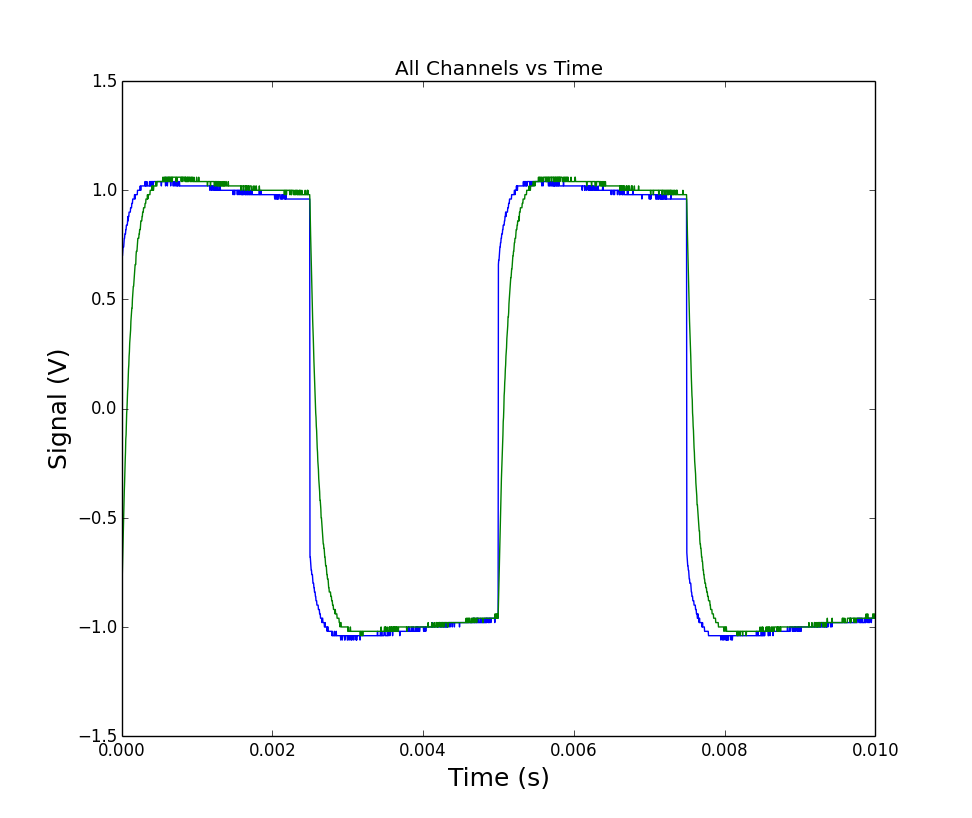
\includegraphics[width=1.5in]{sam_lab2/2g_200hz.png}
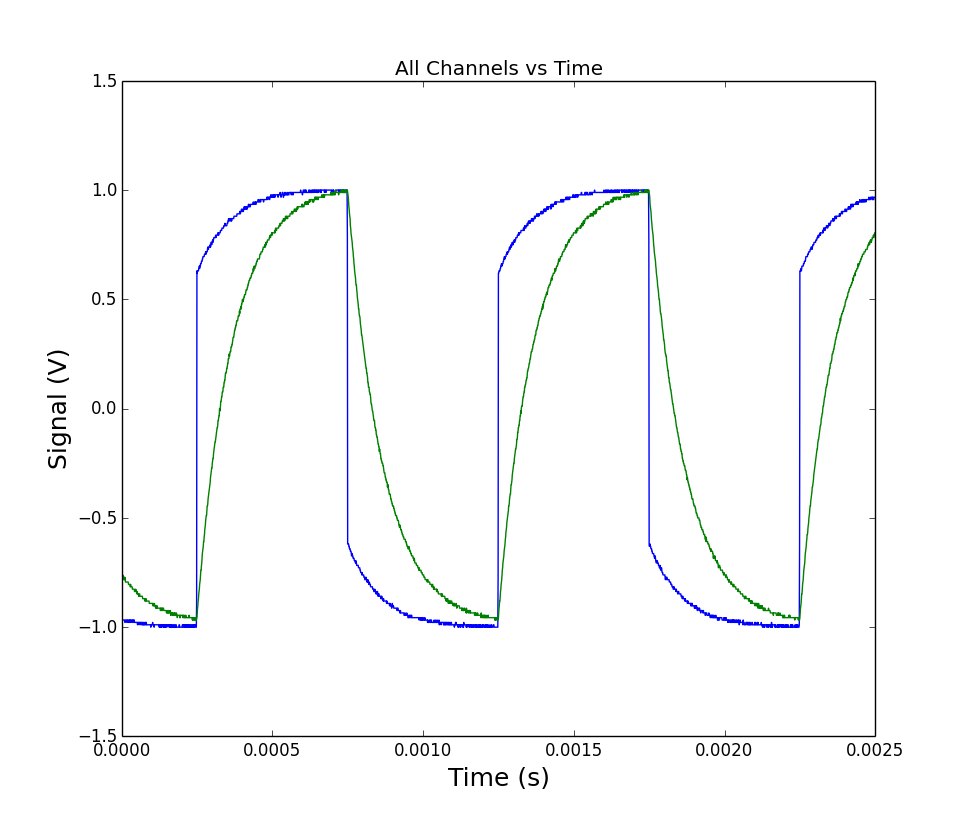
\includegraphics[width=1.5in]{sam_lab2/2g_1kHz.png}
\caption{10 Hz (left) and 200 Hz (middle) show that at these frequencies, almost all of the voltage is being transmitted.  A slight variance can be observed on the 200 Hz plot and a larger variance can be observed on the 1 kHz plot (right).}
\end{figure}
\begin{figure}[h]
\centering
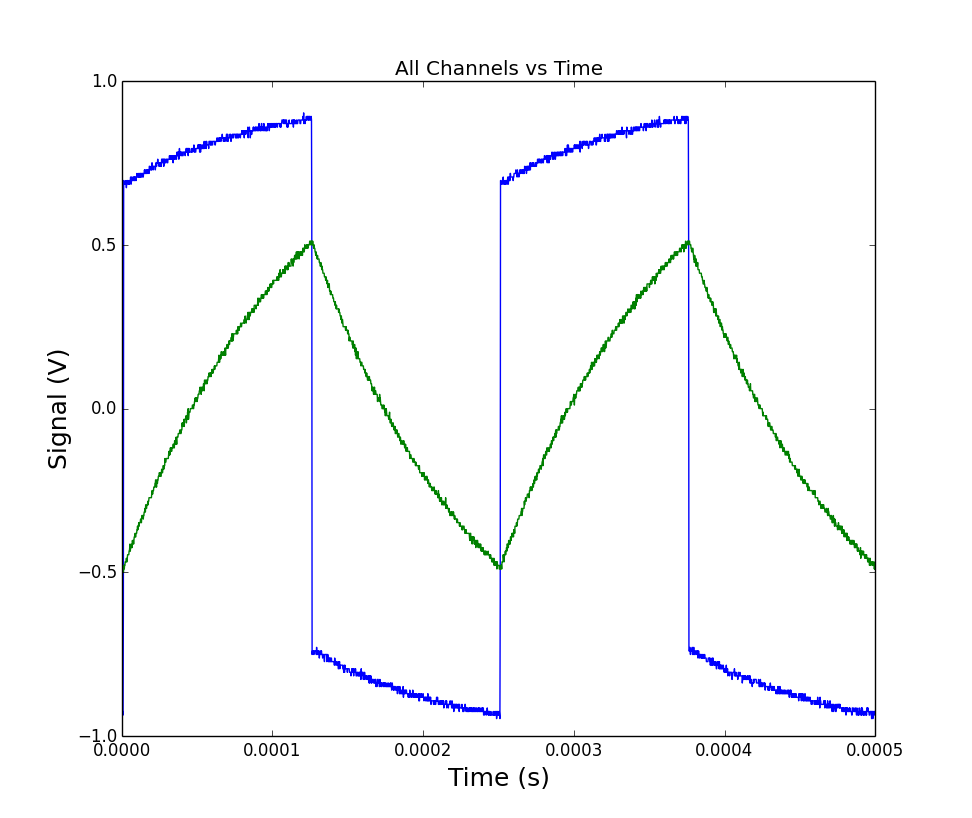
\includegraphics[width=1.5in]{sam_lab2/2g_4kHz.png}
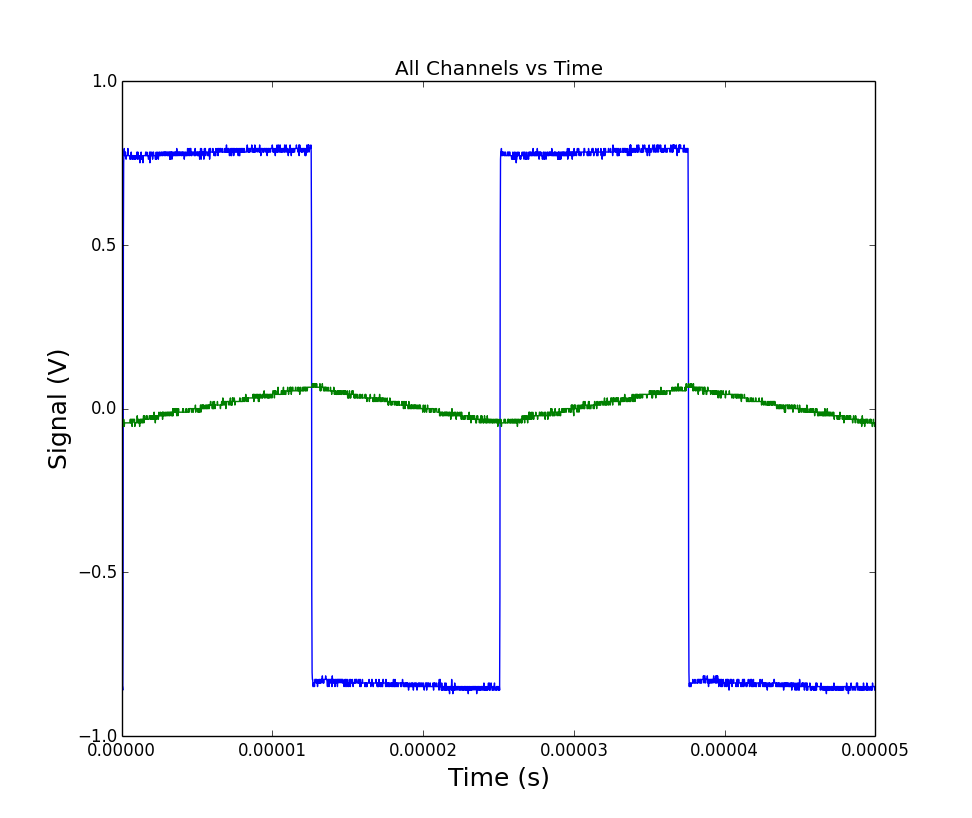
\includegraphics[width=1.5in]{sam_lab2/2g_40kHz.png}
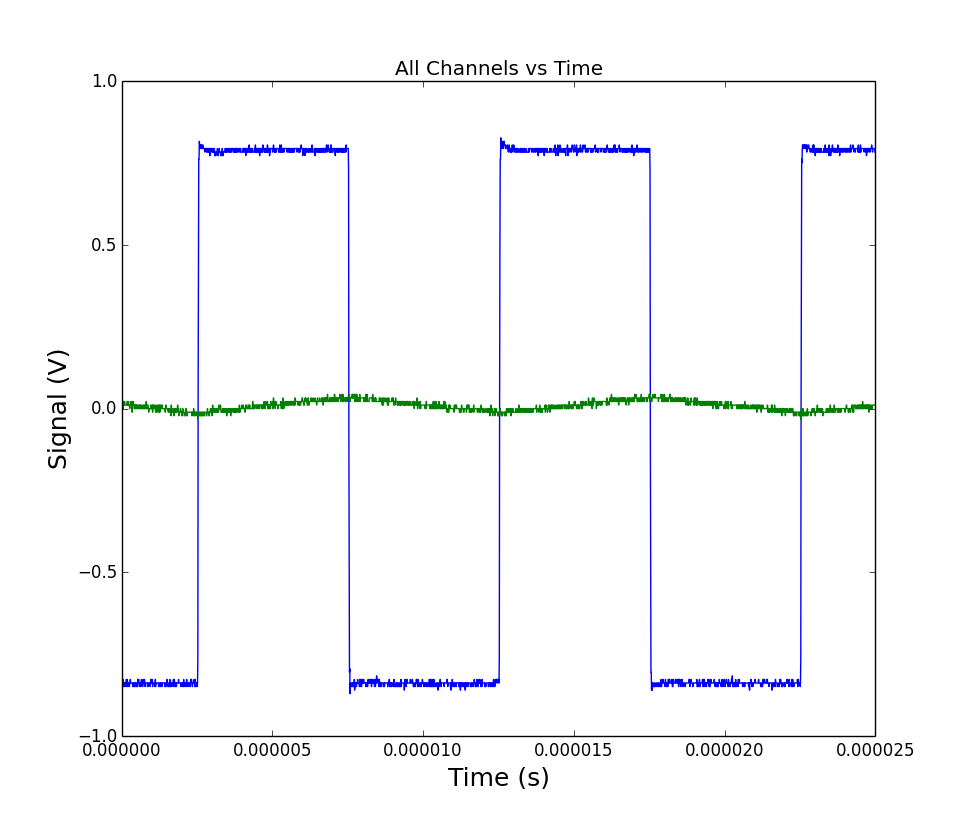
\includegraphics[width=1.5in]{sam_lab2/2g_100kHz.png}
\caption{4 kHz (left) Shows a drastic attenuation happening, while at higher frequencies 40 kHz (middle) and 100 kHz (right) show that almost all the voltage is blocked from the output.}
\end{figure}\\
The plots show that this circuit is a low frequency passing circuit and blocks higher frequencies almost completely.
\newpage
\section*{Experiment 3, The RC Integrator}
\begin{figure}[h]
\centering
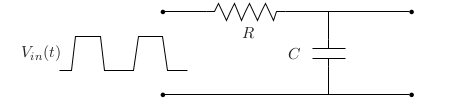
\includegraphics[width=4in]{sam_lab2/3_circuit.png}
\caption{.}
\end{figure}
The circuit used in experiment 2 can be considered an integrator at sufficiently high frequencies.  Looking back at the plots generated for 4 kHz 40 kHz and 100 kHz, the output does indeed look like it could be integrating the input.
\begin{figure}[h]
\centering
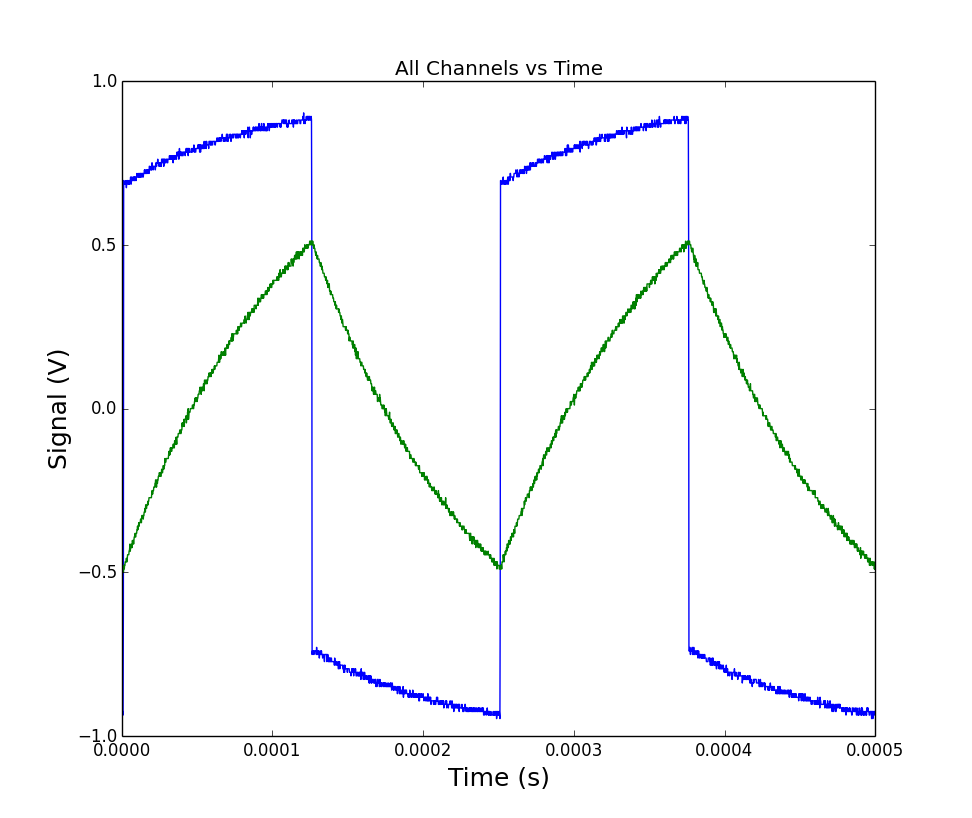
\includegraphics[width=1.5in]{sam_lab2/2g_4kHz.png}
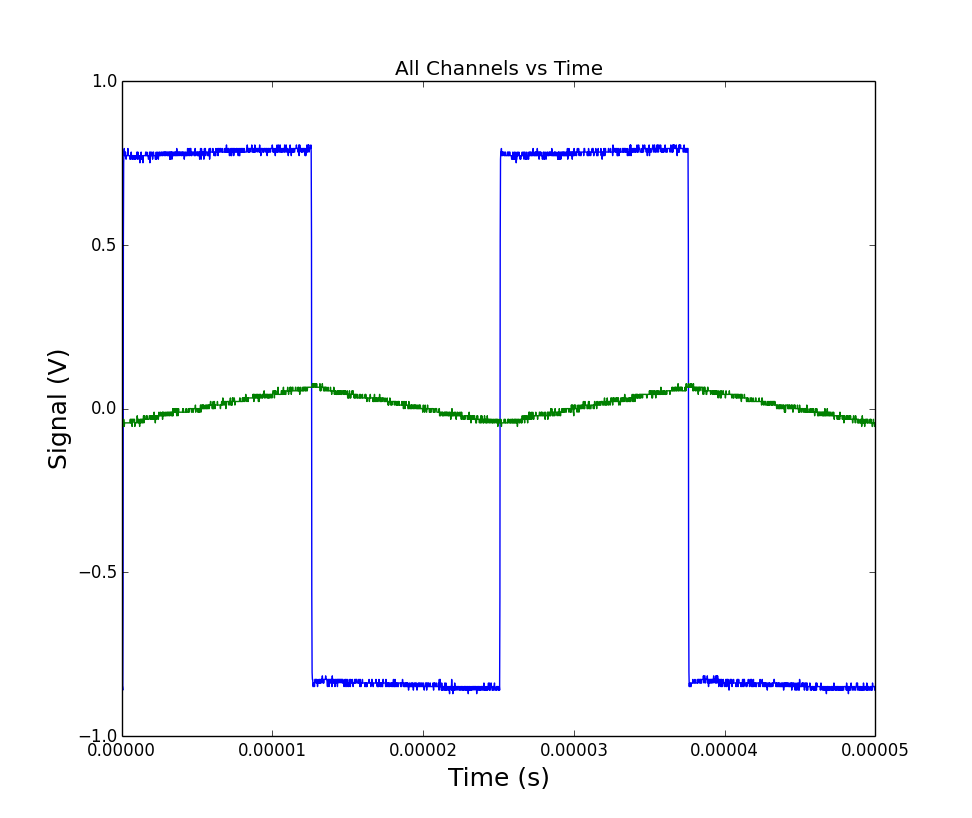
\includegraphics[width=1.5in]{sam_lab2/2g_40kHz.png}
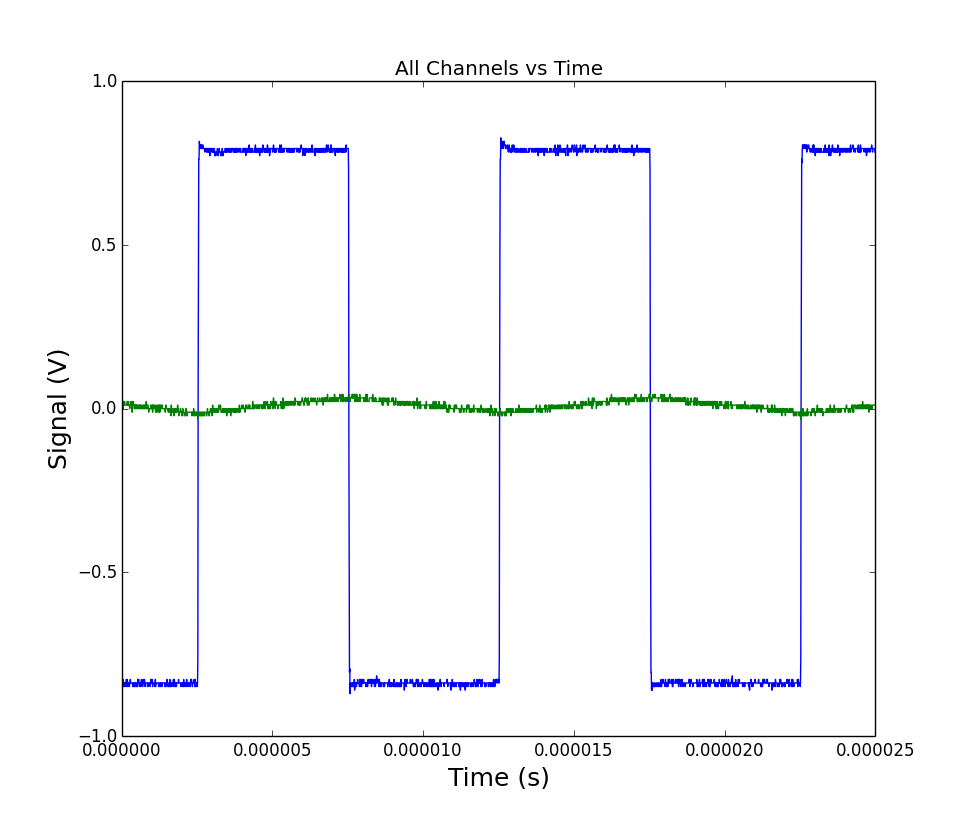
\includegraphics[width=1.5in]{sam_lab2/2g_100kHz.png}
\caption{Observing the integration characteristics shown on the 4 kHz (left) 40 kHz (middle) and 100 kHz (right).  At 4 kHz, the integration appears to be happening, however, there seems to be room for error.}
\end{figure}\\
The circuit seems to be able to make a triangle wave from a square wave input around 40 kHz and bigger, however, the attenuation will get stronger as the frequency goes up. \\
\\
\newpage
\noindent
A 100 kHz triangle wave was applied and the output seems to be sinusoidal.
\begin{figure}[h]
\centering
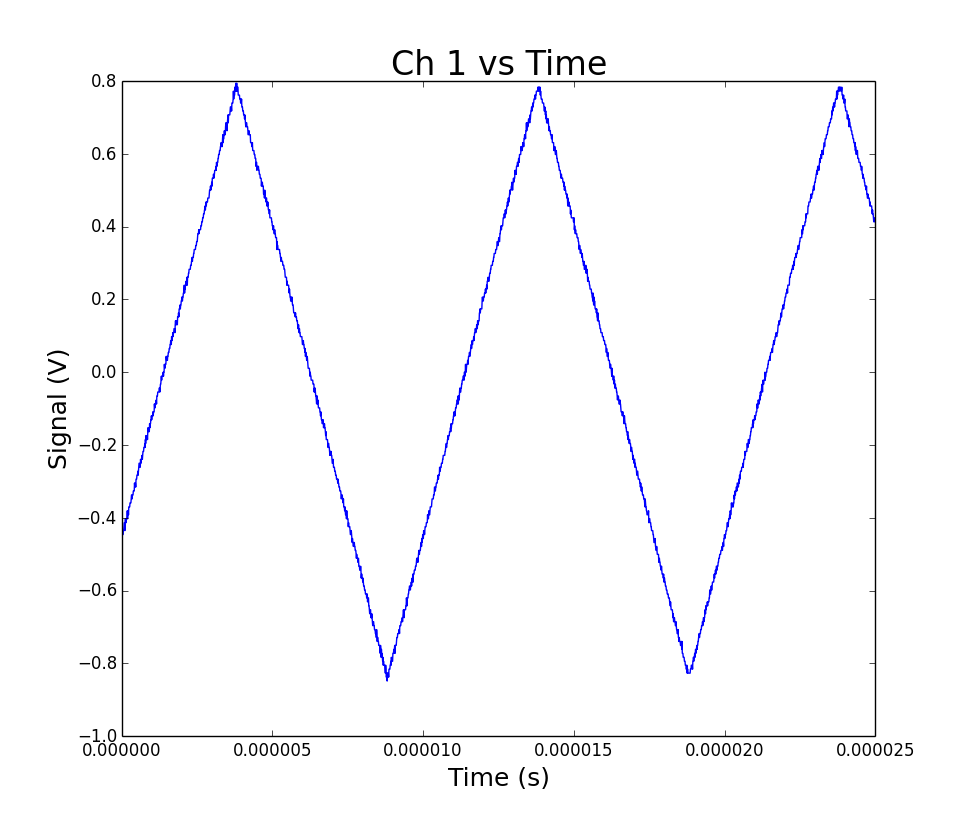
\includegraphics[width=1.5in]{sam_lab2/3d_input.png}
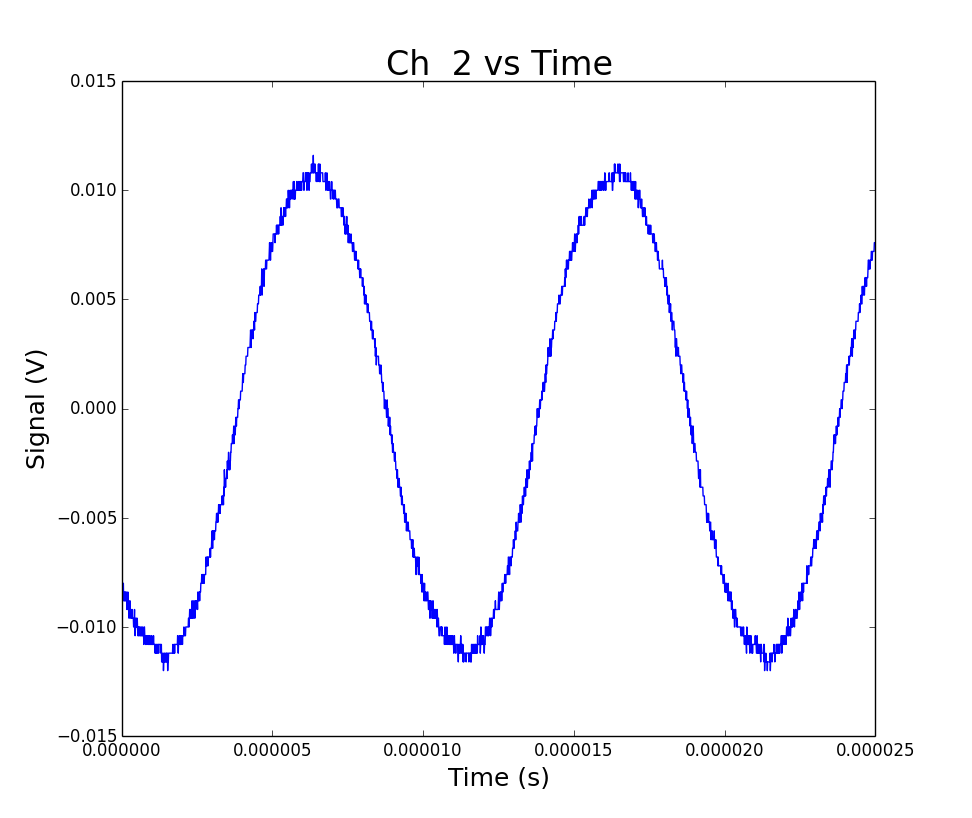
\includegraphics[width=1.5in]{sam_lab2/3d_output.png}
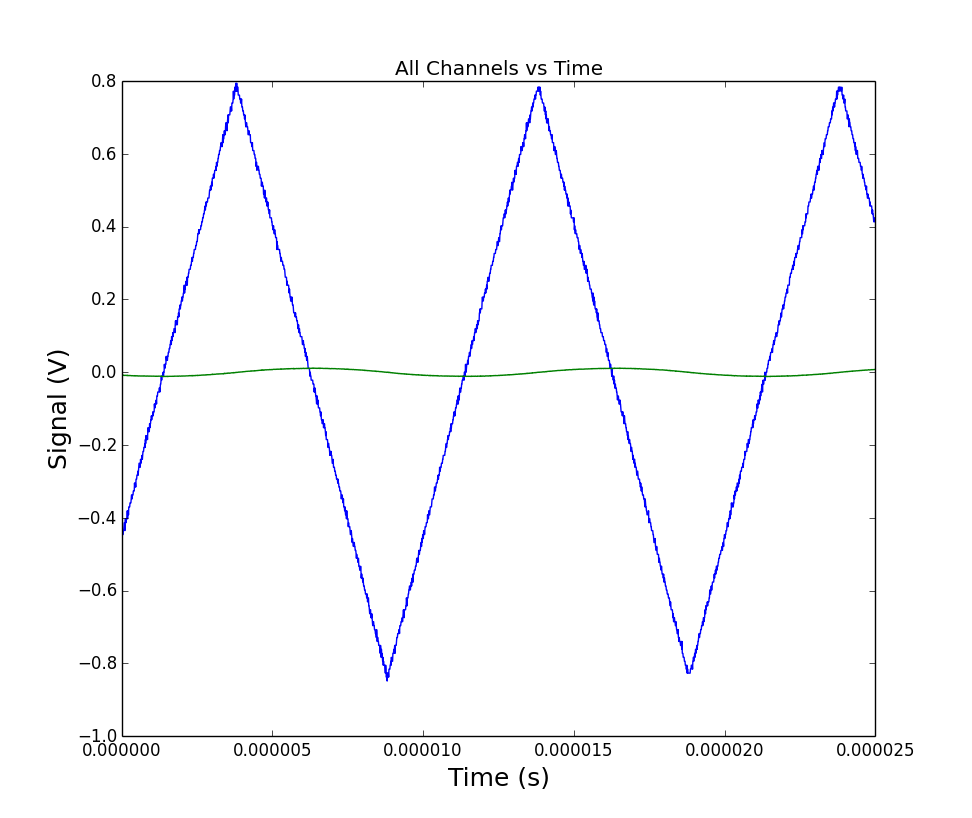
\includegraphics[width=1.5in]{sam_lab2/3d_combined.png}
\caption{100 kHz Triangle wave input (left) `Integrated' `sinusoidal' output (middle) and combined to show attenuation (right). }
\end{figure}\\

\section*{Experiment 4, The CR Configuration}
\begin{figure}[h]
\centering
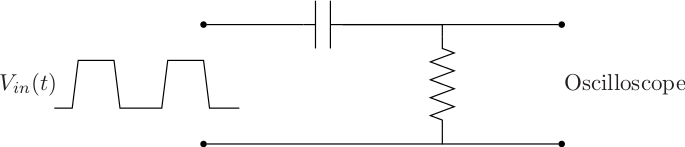
\includegraphics[width=4in]{sam_lab2/4_circuit.png}
\caption{High-pass circuit, using the capacitor and resistor used in experiment 2 and 3 just reversed position.}
\end{figure}
\noindent
The circuit in this experiment was achieved by simply flipping the positive and negative function generator leads around, and moving the ground to the same side as the negative function generator lead.
\\
\\
\newpage
\noindent
A square wave was applied and traces taken at various frequencies.
\begin{figure}[h]
\centering
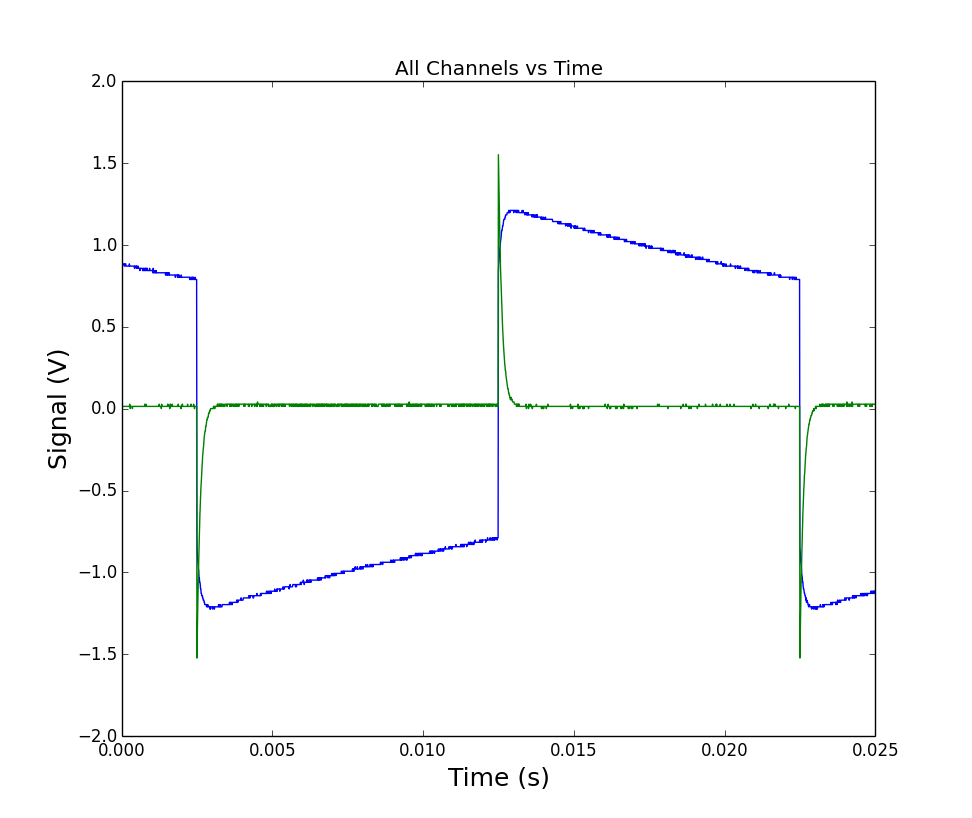
\includegraphics[width=1.5in]{sam_lab2/4b_50Hz.png}
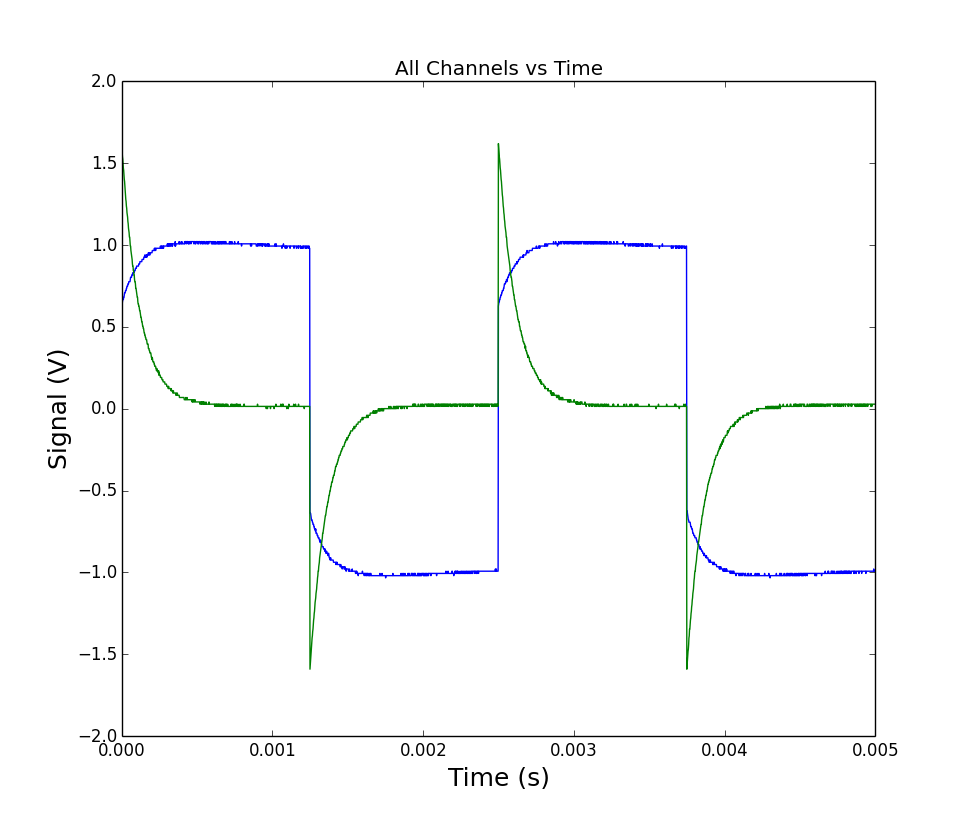
\includegraphics[width=1.5in]{sam_lab2/4b_400Hz.png}
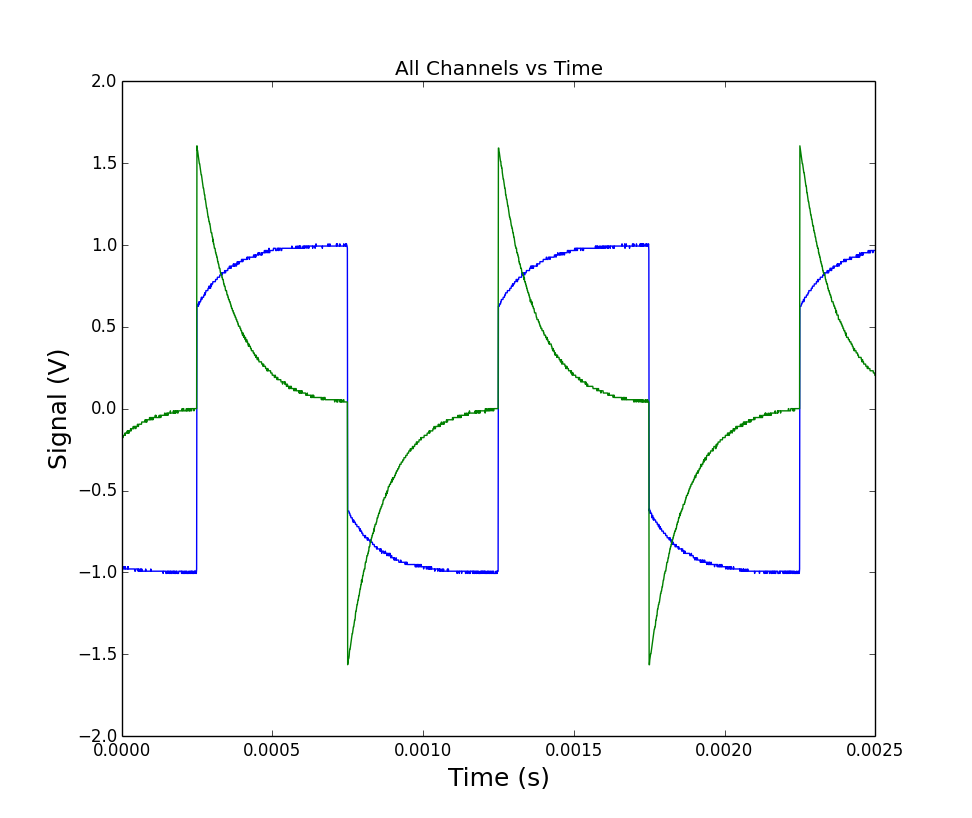
\includegraphics[width=1.5in]{sam_lab2/4b_1kHz.png}
\caption{50 Hz (left), 400 Hz (middle) and 1kHz (right) all show signs of this circuit being a differentiator.  Notice though, that the lower frequencies are experiencing a lot of attenuation.}
\end{figure}\\
\begin{figure}[h]
\centering
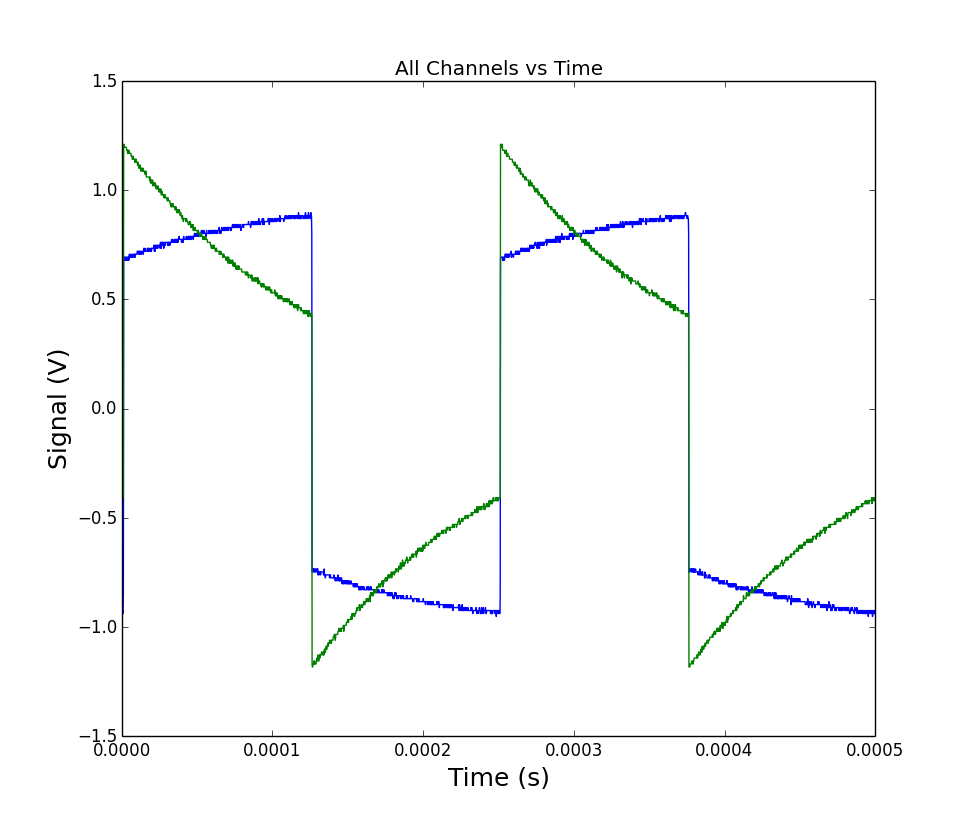
\includegraphics[width=1.5in]{sam_lab2/4b_4kHz.png}
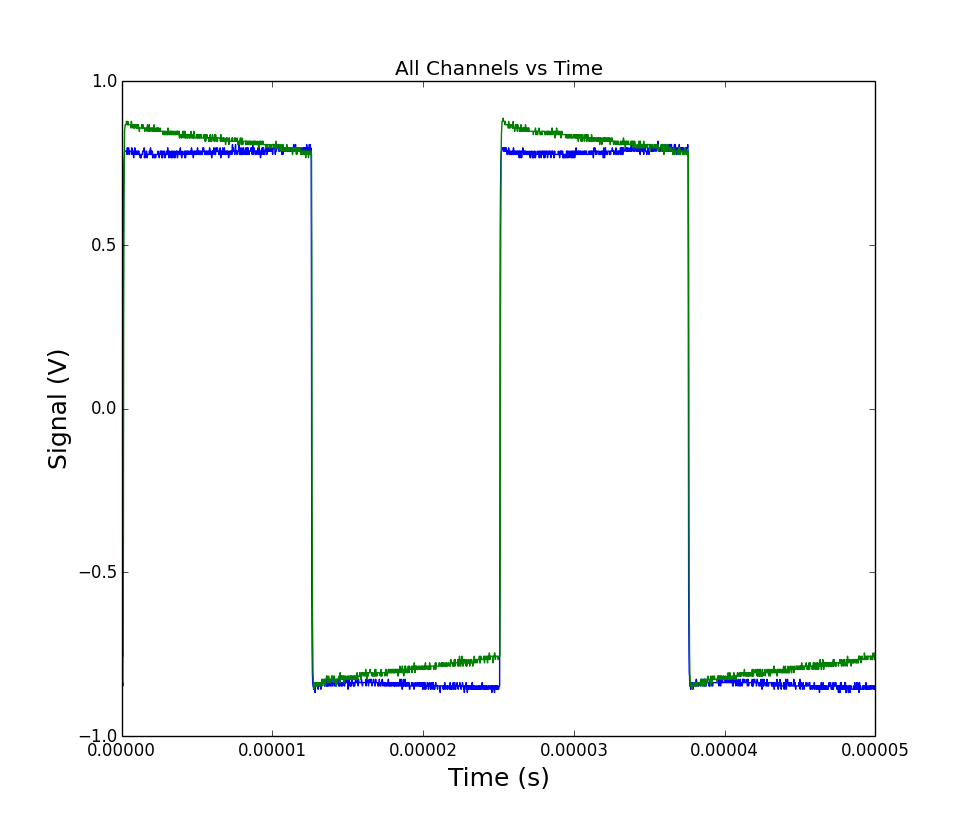
\includegraphics[width=1.5in]{sam_lab2/4b_40kHz.png}
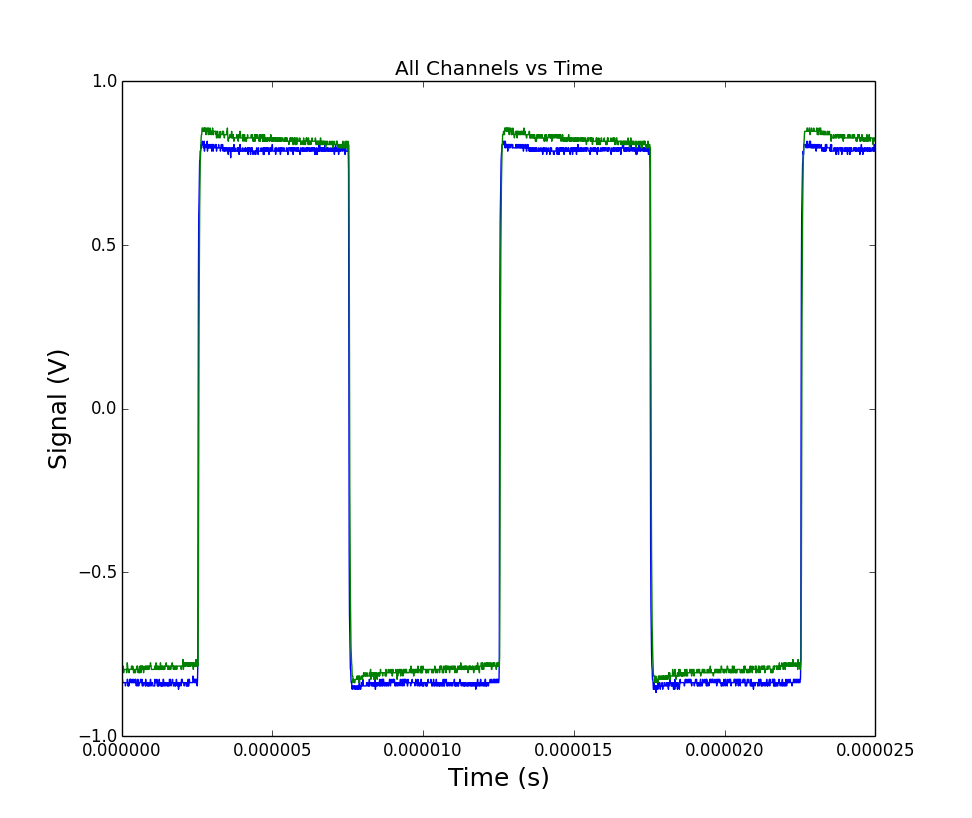
\includegraphics[width=1.5in]{sam_lab2/4b_100kHz.png}
\caption{4 kHz (left) shows some signs of differentiation, however, 40 kHz (middle) and 100 kHz (right) both seem to loose differentiation abilities.  Notice how the circuit lets almost all the Voltage through at the higher frequencies.}
\end{figure}\\
\newpage
A 100 Hz triangle wave was applied to this circuit and differentiation characteristics are noted.  The output looks like a square wave.
\begin{figure}[h]
\centering
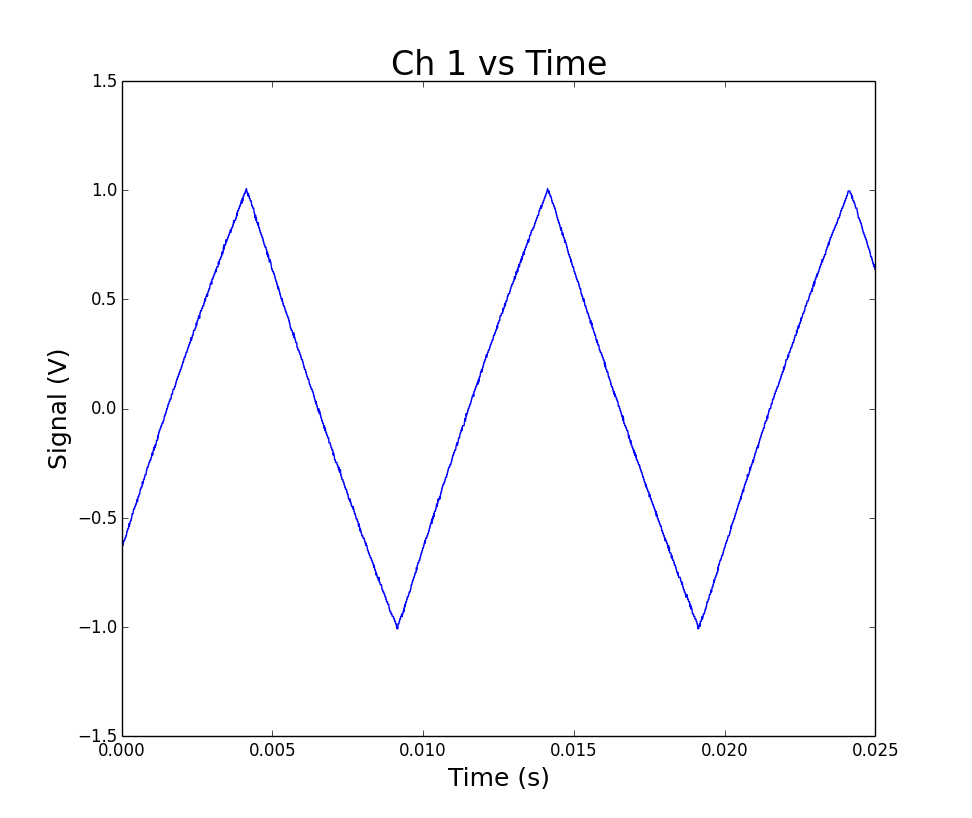
\includegraphics[width=1.5in]{sam_lab2/4c_input.png}
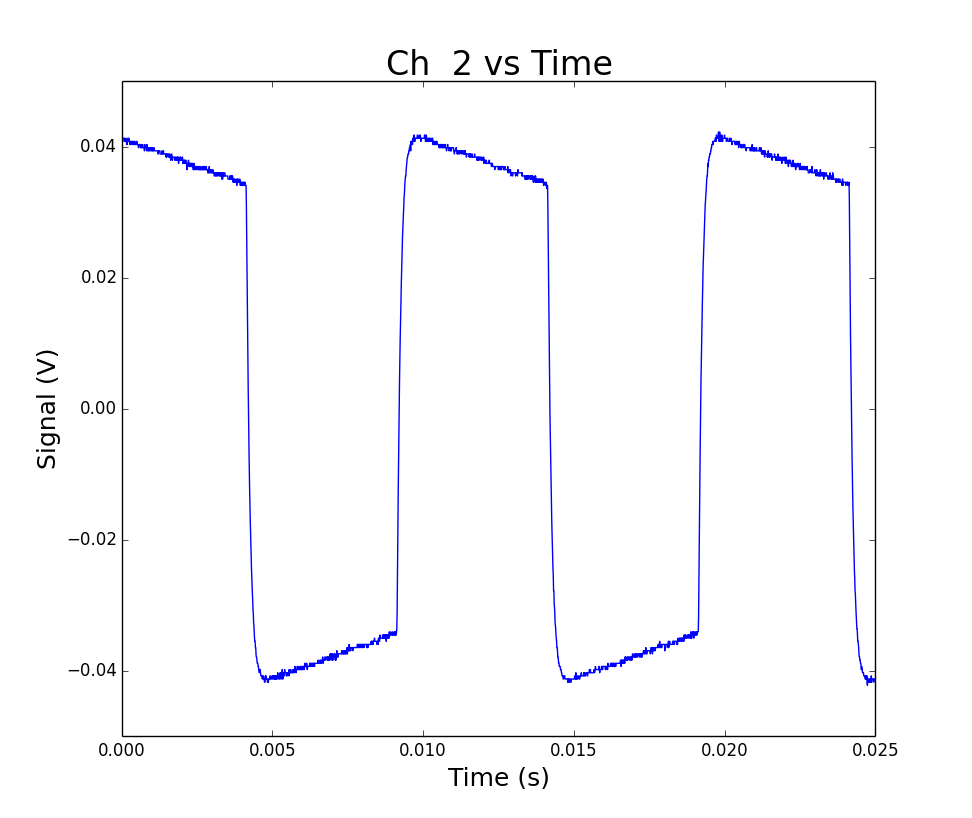
\includegraphics[width=1.5in]{sam_lab2/4c_output.png}
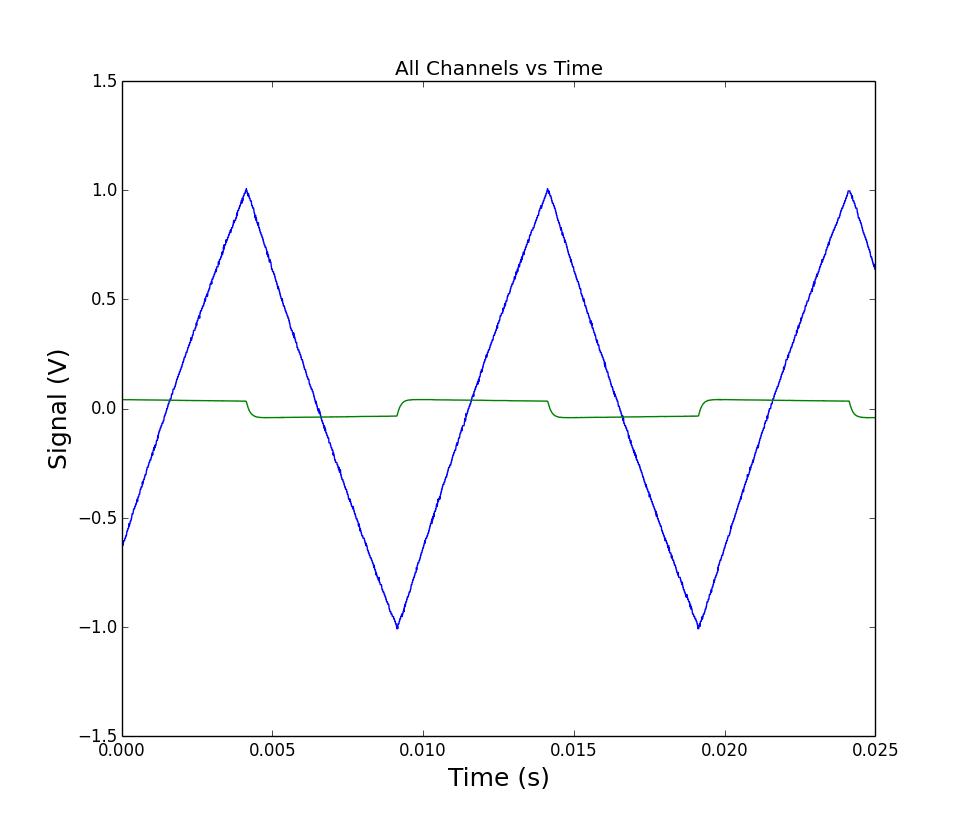
\includegraphics[width=1.5in]{sam_lab2/4c_combined.png}
\caption{100 Hz Triangle wave input(left), squarish wave output (middle) and combined for attenuation (right)}
\end{figure}\\

\end{document}
